% =====================================================================
% q-Weibull Competing Risks under Weak Identifiability:
% Bayesian Inference via the No-U-Turn Sampler
% Target: Quality and Reliability Engineering International (QREI)
% Wiley NJD template (USG class, twocolumn); compile with XeLaTeX.
% =====================================================================
\documentclass[ASNA,twocolumn]{USG}

\usepackage{amsmath,amssymb,amsthm}
\usepackage{bm}
\usepackage{graphicx}
\usepackage{booktabs}
\usepackage{array}
\usepackage{multirow}
\usepackage{tabularx}
\usepackage{algorithm}
\usepackage{algpseudocode}
\usepackage{xcolor}

% proposition / remark environments are provided by the USG class.

\DeclareMathOperator{\CIF}{CIF}
\DeclareMathOperator{\E}{\mathbb{E}}
\DeclareMathOperator{\Var}{\mathrm{Var}}

\begin{document}

\title{q-Weibull Competing Risks under Weak Identifiability: Bayesian
Inference via the No-U-Turn Sampler}

\author[2]{Fuchang Wang}[https://orcid.org/0009-0001-6662-9042]
\author[1]{Huirong Cao}[https://orcid.org/0009-0005-4046-7945]

\authormark{WANG AND CAO}
\titlemark{q-Weibull Competing Risks under Weak Identifiability}

\address[1]{\orgdiv{School of Science, }\orgname{Langfang Normal
University, }\orgaddress{\state{Langfang, }\country{China}}}
\address[2]{\orgname{University of Emergency Management,
}\orgaddress{\state{Sanhe, }\country{China}}}

\corres{Fuchang Wang (\email{wangfuchang@cidp.edu.cn})}

% DOI is assigned by the publisher upon acceptance; left blank in the
% submitted (revision) version so that no placeholder DOI is printed.
\articledoi{}

\keywords{q-Weibull distribution | competing risks | weak identifiability |
Bayesian inference | No-U-Turn Sampler}

\abstract[ABSTRACT]{Competing-risks data, where each unit fails from one
of several mutually exclusive causes, arise routinely in reliability and
lifetime analysis. The q-Weibull distribution nests the ordinary Weibull
and accommodates both bounded ($q<1$) and heavy-tailed ($q>1$) lifetimes,
but Bayesian inference for it under competing risks remains
under-developed. We develop a unified Bayesian framework computed by the
No-U-Turn Sampler (NUTS) in a more weakly coupled, unconstrained
coordinate system $(q,\log\eta,\log\beta)$, with an analytic gradient,
Hessian-based preconditioning, and a smooth barrier at the bounded
support wall. Because early competing failures remove the tail
observations from which $q$ is learned, competing truncation leaves $q$
weakly identifiable: the profile likelihood is broad and Wald intervals
under-cover. Across six shape values spanning the bounded, Weibull, and
heavy-tailed regimes and three truncation levels, we show that,
\emph{specifically under strong competing-risk truncation and when the
true $q$ is moderately close to the regularising centre}, a quadratic $q$
penalty (prior shrinkage) reduces the root-mean-squared error and
restores near-nominal coverage. A controlled comparison with unpenalised
MLE, penalised MLE, and the mode (MAP) shows that most of this
point-estimate gain is attributable to the regularisation itself rather
than to Bayesian computation; the added value of the full Bayesian
analysis is calibrated posterior intervals, whose coverage we document.
When the tail is observed or $q$ lies far from the prior centre, the
likelihood dominates and the MLE is preferable. NUTS adapts its mass
matrix automatically and uses gradient evaluations about twice as
efficiently as fixed-trajectory HMC, and its effective-sample throughput
is comparable to a mature probabilistic-programming implementation on the
same data. On high-voltage stress-test data ($n=58$), competing risks are
significant, but the early mode shows only an uncertain heavy-tail
signal, and posterior predictive checks are consistent with the observed
lifetimes; the degradation mode is well described by an ordinary
Weibull.}

\maketitle

\vspace{1em}

% =====================================================================
\section{Introduction}\label{sec:intro}
% =====================================================================

Competing risks occur when a unit is exposed to several mutually exclusive
failure mechanisms and the observed lifetime is the minimum of the latent
cause-specific times, together with an indicator of the cause responsible.
Such data are routine in the analysis of electronic components, mechanical
systems, and accelerated life tests \cite{crowder2001,pintilie2006}. Because failure by one cause removes
the unit from exposure to all others, the latent times of the non-operating
causes are censored, a structure that must be respected by both the
likelihood and any inferential procedure.

The Weibull distribution has long been the workhorse of parametric
reliability analysis. Its fixed stretched-exponential tail, however, cannot
represent
the heavier-than-Weibull tails associated with wear-out heterogeneity, nor
the finite upper support that arises for certain bounded-failure processes.
The q-Weibull distribution, obtained from Tsallis entropy
\cite{tsallis1988} and studied in reliability by several authors
\cite{costa2006,jose2009}, nests the ordinary Weibull at $q=1$, gives a
heavy (power-law) tail for $1<q<2$, and a bounded support for $q<1$. A single
additional parameter thus extends the Weibull in two useful directions.

Despite this flexibility, inference for q-Weibull competing risks faces
three difficulties. \emph{First}, the parameter that governs the tail, $q$,
is identified largely from observations in the tail; when a competing cause
truncates the lifetime distribution early, the tail of the cause of interest
is only partially observed and $q$ can become weakly identifiable, with a
profile likelihood that is broad, flat, or asymmetric. \emph{Second},
maximum-likelihood estimates and their Wald standard errors rely on local
quadratic and asymptotic-normal approximations that are unreliable in this
limited-information regime, and the bounded regime introduces a hard support
boundary at which the log-density is singular. \emph{Third}, generic
random-walk Metropolis samplers mix poorly over the correlated, curved
q-Weibull parameter space, making a naive Bayesian implementation
computationally expensive.

This article addresses all three difficulties with a unified Bayesian
treatment computed by the No-U-Turn Sampler (NUTS)
\cite{hoffman2014nuts}, an adaptive form of Hamiltonian Monte Carlo (HMC)
\cite{neal2011,betancourt2017} that uses gradient information and recursive
trajectory doubling. Recent work has applied HMC to Weibull-based competing
risks \cite{abba2025wdcr,abdullahi2026,bfm2025}, used NUTS for Bayesian
inference of short- and long-tailed queueing models \cite{alawamy2025}, and
applied Gibbs sampling to the q-Weibull \cite{sigma2026gibbs}. The same
high-voltage endurance data have been analysed with ordinary Weibull
competing risks under adaptive progressive censoring \cite{elshahhat2024}.
The present framework differs by targeting the q-Weibull directly, by using
NUTS rather than Gibbs or random-walk proposals, and by treating
identifiability under competing truncation as a first-class question. Our
contributions are:
\begin{enumerate}
  \item We establish a \textbf{Bayesian framework for q-Weibull competing
  risks under partially observed tails}, formulated in unconstrained,
  weakly coupled coordinates $(q,\log\eta,\log\beta)$, with a
  cause-separable likelihood and an analytic log-posterior gradient that
  remains valid continuously across $q=1$.
  \item We \textbf{characterise the loss of identifiability of $q$ induced by
  competing-risk truncation}: early competing failures remove the tail
  observations from which $q$ is learned, giving broad, flat, or asymmetric
  profile likelihoods, and we document how this affects the bounded and
  heavy-tailed regimes differently.
  \item We develop a \textbf{computational strategy} combining an
  unconstrained parameterisation, analytic gradients, Hessian
  preconditioning, and a smooth treatment of the bounded-support wall and the
  parameter bounds, so that Hamiltonian trajectories explore the posterior
  without entering singular regions.
  \item Through an \textbf{extensive simulation over the bounded, Weibull, and
  heavy-tailed regimes}, we show that Bayesian regularisation improves
  root-mean-squared error and interval coverage specifically in the weakly
  identified, strongly truncated regime, whereas the likelihood dominates
  when the tail is observed.
  \item We give a \textbf{reliability application} that shows how the
  framework distinguishes genuine evidence for a heavy tail from a mere
  displacement of the posterior above $q=1$, avoiding over-interpretation of
  a small, heavily censored sample.
\end{enumerate}

The remainder of the article is organised as follows. Section
\ref{sec:qw} defines the q-Weibull distribution and its properties.
Section \ref{sec:cr} develops the competing-risks model, likelihood, and
derived quantities. Section \ref{sec:bayes} presents the Bayesian
formulation, and Section \ref{sec:nuts} the NUTS computation including the
smooth barrier and diagnostics. Sections \ref{sec:sim} and
\ref{sec:app} report the simulation study and the high-voltage application,
respectively. Section \ref{sec:disc} discusses the findings, and Section
\ref{sec:concl} concludes.

% =====================================================================
\section{The q-Weibull distribution}\label{sec:qw}
% =====================================================================

A q-Weibull random variable $T>0$ has survival function
\begin{equation}\label{eq:R}
R(t) = \Pr(T>t)
     = \big[\,1-(1-q)\,\lambda\, t^{\beta}\,\big]^{\frac{2-q}{1-q}},
\end{equation}
where $\beta>0$ is a shape parameter, $\lambda>0$ a scale-related parameter,
and $q<2$ the entropic shape parameter. Define the \emph{inner factor}
\begin{equation}\label{eq:inner}
u(t) := 1-(1-q)\,\lambda\, t^{\beta}.
\end{equation}
The probability density and hazard functions are
\begin{align}
f(t) &= (2-q)\,\beta\,\lambda\,t^{\beta-1}\,
       u(t)^{\frac{1}{1-q}}, \label{eq:f}\\
h(t) &= \frac{(2-q)\,\beta\,\lambda\,t^{\beta-1}}{u(t)}. \label{eq:h}
\end{align}
It is convenient to express the scale through the characteristic life
$\eta>0$, setting
\begin{equation}\label{eq:lam}
\lambda = \eta^{-\beta}.
\end{equation}

\subsection{Parameter regimes}
Equation \eqref{eq:R} contains three regimes.
\begin{itemize}
  \item \emph{Ordinary Weibull ($q\to1$).} Taking the limit,
  $R(t)\to\exp(-\lambda t^\beta)=\exp[-(t/\eta)^\beta]$, the standard
  two-parameter Weibull survival function.
  \item \emph{Heavy tail ($1<q<2$).} Here $1-q<0$, so $u(t)=1+(q-1)\lambda
  t^\beta>1$ for all $t$ and the support is unbounded. The survival function
  decays as a power law, $R(t)\asymp t^{-\beta(2-q)/(q-1)}$, giving a tail
  heavier than the Weibull's stretched exponential.
  \item \emph{Bounded support ($q<1$).} Here $u(t)$ reaches zero at the finite
  upper endpoint
  \begin{equation}\label{eq:Tmax}
  T_{\max} = \left[\frac{1}{(1-q)\lambda}\right]^{1/\beta}
           = \eta\,(1-q)^{-1/\beta},
  \end{equation}
  so that $R(t)=0$ for $t\ge T_{\max}$.
\end{itemize}

\begin{remark}[Asymmetric identifiability]
As shown empirically in Section \ref{sec:sim}, the heavy-tail parameter
$q>1$ is identified by the tail decay rate and is estimable when the tail is
observed, whereas for $q<1$ the parameters $(q,\beta,T_{\max})$ are strongly
coupled over the observed range and $q$ is only weakly identifiable. This
asymmetry motivates both the simulation design and the Bayesian
regularisation developed below.
\end{remark}

% =====================================================================
\section{Competing risks model}\label{sec:cr}
% =====================================================================

Consider $K$ mutually exclusive failure causes with latent cause-specific
lifetimes $T_1,\dots,T_K$, independently distributed with cause-specific
survival functions $R_j(t)$. The observed data on each unit are
\begin{equation}\label{eq:obs}
T = \min_{1\le j\le K} T_j, \qquad
C = \arg\min_{1\le j\le K} T_j,
\end{equation}
with right-censoring indicated when the unit has not failed by the
censoring time.

\subsection{Cause-specific likelihood}
For a unit failing from cause $j$ at time $t$, the density is
$f_j(t)\prod_{\ell\ne j}R_\ell(t)$: cause $j$ occurs in $(t,t+dt)$ while all
other causes survive beyond $t$. A unit right-censored at $t$ contributes
$\prod_{j=1}^K R_j(t)$. Hence for data $(t_i,c_i)$, with $c_i=j$ for a
cause-$j$ failure and $c_i=0$ (sentinel) for censoring, the likelihood is
\begin{equation}\label{eq:L}
\mathcal{L} =
\prod_{i:\,c_i=j} f_j(t_i)\!\!\prod_{\ell\ne j}\!\!R_\ell(t_i)
\;\prod_{i:\,\mathrm{censored}}\prod_{j=1}^K R_j(t_i).
\end{equation}
Taking logarithms, the log-likelihood \emph{separates by cause}. The
contribution of cause $j$ is
\begin{equation}\label{eq:Lj}
\ell_j(\bm\theta_j)
 = \sum_{i:\,c_i=j}\log f_j(t_i)
 + \sum_{i:\,c_i\ne j}\log R_j(t_i),
\end{equation}
where the second sum includes both failures from other causes and censored
units (for which cause $j$ is right-censored). Thus
$\log\mathcal{L}=\sum_{j=1}^K \ell_j$, and each cause may be fitted using a
single-distribution routine in which its own failures are events and all
other observations are right-censored.

\subsection{System survival and cumulative incidence functions}
The system survival and system density are
\begin{equation}\label{eq:Rsys}
R_{\mathrm{sys}}(t)=\prod_{j=1}^K R_j(t), \qquad
f_{\mathrm{sys}}(t)=\sum_{j=1}^K f_j(t)\prod_{\ell\ne j}R_\ell(t).
\end{equation}
The cumulative incidence function (CIF) for cause $j$, the probability of
failure from cause $j$ by time $t$ in the presence of all other causes, is
\begin{equation}\label{eq:cif}
\CIF_j(t)=\int_0^t f_j(s)\prod_{\ell\ne j}R_\ell(s)\,ds.
\end{equation}
The CIFs partition the failure probability:
\begin{equation}\label{eq:cif-id}
\sum_{j=1}^K \CIF_j(t)=1-R_{\mathrm{sys}}(t).
\end{equation}
The eventual (crude) probability of cause $j$ is $\CIF_j(\infty)$. In the
numerical work \eqref{eq:cif} is evaluated by trapezoidal integration on a
fine time grid, and identity \eqref{eq:cif-id} provides a numerical check.
To confirm numerical stability, the CIFs and system reliability were
recomputed on grids of $500$, $1000$, $5000$, and $10\,000$ points: the
posterior summaries changed by less than $10^{-3}$ once the grid reached
$1000$ points, and all results below use a $5000$-point grid.

% =====================================================================
\section{Bayesian formulation}\label{sec:bayes}
% =====================================================================

\subsection{Parameterisation and priors}\label{sec:param}
Direct sampling in $(\lambda,\beta)$ is ill-conditioned because
$\log\lambda=-\beta\log\eta$ couples the scale and shape, and the bounded
regime adds a hard support constraint. We instead work in the unconstrained,
weakly coupled coordinates
\begin{equation}\label{eq:x}
\bm{x}=(x_q,x_e,x_b), \qquad
q=2-e^{x_q},\quad \eta=e^{x_e},\quad \beta=e^{x_b},
\end{equation}
with $\lambda=\eta^{-\beta}$ derived. The transformation for $q$ is
monotone from $\mathbb{R}$ to $(-\infty,2)$, and those for $\eta,\beta$ to
$(0,\infty)$, so no constrained sampling is required.

Independent weakly informative priors are placed on the natural parameters
\begin{equation}\label{eq:prior}
q\sim\mathcal{N}(\mu_q,\sigma_q^2),\quad
\log\eta\sim\mathcal{N}(\mu_e,\sigma_e^2),\quad
\log\beta\sim\mathcal{N}(\mu_b,\sigma_b^2),
\end{equation}
with the $q$ prior truncated to the admissible range. We use a data-driven
default: $\mu_e=\log(\mathrm{median\ event\ time})$, $\sigma_e=1.5$;
$\mu_b=\log 1.5$, $\sigma_b=1.2$; and $\mu_q=1$ (the ordinary Weibull as the
regularising centre) with $\sigma_q=0.5$ for competing-risks analysis. The
scale priors are deliberately broad so that, when the data are informative,
the likelihood dominates; the $q$ prior's role is to regularise the
limited-information tail parameter (Section \ref{sec:sim}).

We deliberately \emph{do not} claim that $(q,\log\eta,\log\beta)$ is
orthogonal. A natural alternative is $(q,\log\lambda,\log\beta)$, in which
$\log\lambda=-\beta\log\eta$ might be expected to decouple scale from
shape. We tested both parameterisations quantitatively on the voltage
posterior, at the posterior mode, by the Hessian condition number
$\kappa(\bm H)$, the effective samples per second, the number of
divergences, mean tree depth, and $\hat R$ (Figure~\ref{fig:parcorr},
Table~\ref{tab:parparam}). The proposed coordinates give
$\kappa\approx1.75\times10^{3}$, $129.5$ effective samples per second,
$18$ divergent transitions, mean tree depth $1.94$, and $\hat R_{\max}=1.004$,
whereas $(q,\log\lambda,\log\beta)$ gives $\kappa\approx9.66\times10^{5}$
(about $550$ times worse), $0.061$ effective samples per second, $26$
divergences, mean tree depth $5.74$, and $\hat R_{\max}=1.17$, which
fails to converge. We therefore find \emph{no evidence} that
$(q,\log\lambda,\log\beta)$ is the more orthogonal parameterisation; it is
strictly worse, because $\log\lambda$ remains strongly coupled to $\beta$
through $\log\lambda=-\beta\log\eta$. We keep $(q,\log\eta,\log\beta)$ and
describe it as merely a \emph{more weakly coupled} unconstrained
system. The largest posterior correlation in our chosen coordinates is
$|\rho|\approx0.94$, confined within a single failure mode's
scale--shape block, and is absorbed by the Hessian preconditioner of
Section~\ref{sec:adapt}.

\begin{table}[h]
\centering
\caption{Comparison of the proposed $(q,\log\eta,\log\beta)$
parameterisation (A) against $(q,\log\lambda,\log\beta)$ (B) on the
voltage posterior, evaluated at the posterior mode.}
\label{tab:parparam}
\small
\begin{tabular}{lcc}
\toprule
Quantity & A: $(q,\log\eta,\log\beta)$ & B: $(q,\log\lambda,\log\beta)$\\
\midrule
Hessian condition number $\kappa(\bm H)$ & $1.75\times10^{3}$ & $9.66\times10^{5}$\\
Effective samples / second & $129.5$ & $0.061$\\
Divergent transitions (sampling) & $18$ & $26$\\
Mean tree depth & $1.94$ & $5.74$\\
$\hat R_{\max}$ & $1.004$ & $1.17$\\
\bottomrule
\end{tabular}
\end{table}

\begin{figure}[h]
\centering
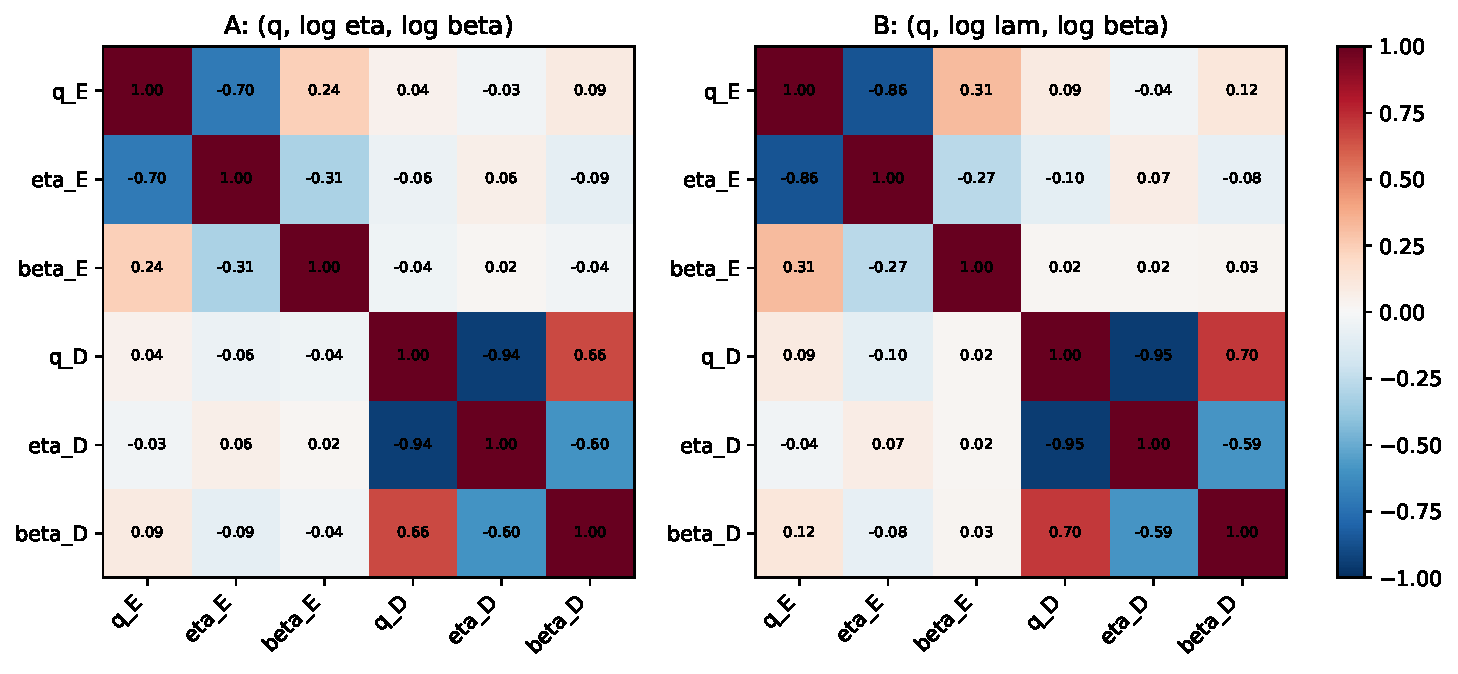
\includegraphics[width=\linewidth]{../figures/fig8_param_corr.pdf}
\caption{Posterior correlation structure (parametric comparison). The
alternative $(q,\log\lambda,\log\beta)$ parameterisation (B) is not more
orthogonal: its Hessian is about $550$ times worse-conditioned and its
chains fail to converge. We therefore retain $(q,\log\eta,\log\beta)$ and
describe it only as a more weakly coupled system.}
\label{fig:parcorr}
\end{figure}

\subsection{Posterior and analytic gradient}\label{sec:post}
Because the priors in \eqref{eq:prior} are expressed in the natural
coordinates while sampling is in $\bm{x}$, the change of variables for
$q=2-e^{x_q}$ contributes the Jacobian term
$\log|\partial q/\partial x_q|=x_q$; the priors on $\log\eta,\log\beta$ are
already on $x_e,x_b$. The log-posterior is
\begin{equation}\label{eq:post}
\log p(\bm{x}\mid\text{data})
 = \ell(\bm{x})
 -\frac12\Big(\frac{q-\mu_q}{\sigma_q}\Big)^2 + x_q
 -\frac12\Big(\frac{x_e-\mu_e}{\sigma_e}\Big)^2
 -\frac12\Big(\frac{x_b-\mu_b}{\sigma_b}\Big)^2 .
\end{equation}

Let $g_q,g_\lambda,g_\beta$ denote the derivatives of the log-likelihood
with respect to the raw parameters $(q,\lambda,\beta)$, obtained
analytically. Chaining through \eqref{eq:x} and $\lambda=\eta^{-\beta}$,
\begin{equation}\label{eq:chain}
\frac{\partial\ell}{\partial x_e}=-\beta\,\lambda\,g_\lambda,
\qquad
\frac{\partial\ell}{\partial x_b}
 =\beta\big(g_\beta-g_\lambda\lambda x_e\big),
\qquad
\frac{\partial\ell}{\partial x_q}=-e^{x_q}g_q .
\end{equation}
The likelihood is differentiable at $q=1$. Writing $z=\lambda t^\beta$, the
limiting $q$-derivative is
\begin{equation}\label{eq:q1lim}
g_q\big|_{q=1} =
\sum_{\mathrm{events}}\Big(\frac{z^2}{2}-1\Big)
+\sum_{\mathrm{censored}}\Big(z+\frac{z^2}{2}\Big).
\end{equation}
The analytic gradient \eqref{eq:chain} agrees with a numerical gradient to
relative error below $10^{-8}$, and the cause-separable form
\eqref{eq:Lj} lets the competing-risks posterior reuse the single-cause
routine for each mode.

% =====================================================================
\section{NUTS computation}\label{sec:nuts}
% =====================================================================

\subsection{Hamiltonian dynamics and the No-U-Turn Sampler}\label{sec:hmc}
HMC augments the state with an auxiliary momentum $\bm r$ and defines the
Hamiltonian
\begin{equation}\label{eq:H}
H(\bm{x},\bm r)=-\log p(\bm{x})+\tfrac12\bm r^\top\bm M^{-1}\bm r,
\end{equation}
where $\bm M$ is a mass (preconditioning) matrix. The canonical equations
are simulated by the leapfrog integrator, which alternates half-kicks in
momentum and full steps in position. The No-U-Turn Sampler builds a
balanced binary trajectory by recursively doubling the leapfrog path in a
randomly chosen direction, stopping when the path doubles back on itself (a
U-turn), when a divergence is detected, or at a maximum tree depth; a
slice variable provides a valid, detailed-balance-preserving proposal over
the valid points, as implemented in Stan \cite{carpenter2017stan}. Algorithm
\ref{alg:nuts} summarises the procedure.

\begin{algorithm}[t]
\caption{NUTS for q-Weibull (competing risks), with Hessian mass and
dual-averaging step size}
\label{alg:nuts}
\begin{algorithmic}[1]
\Require data $(t_i,c_i)$; initial point $\bm x_0$; target acceptance
$\delta$; draws $N$, warmup $W$
\State $\bm M \gets \mathrm{regularize}(-\nabla^2\log p(\bm x_0))$;
$\bm M^{-1}$; $\bm L\gets\mathrm{chol}(\bm M)$
\State choose step size $\varepsilon$ by the find-reasonable-epsilon routine
\For{$m=1$ \textbf{to} $N+W$}
  \State draw $\bm r\sim\mathcal{N}(\bm0,\bm M)$;
  $\log u\gets \log p(\bm x)-\tfrac12\bm r^\top\bm M^{-1}\bm r+\log U$
  \State recursively double the trajectory (both directions) until a
  U-turn, divergence, or max depth; track valid points
  \State set $\bm x$ to a slice-weighted valid point; flag a divergence if
  the energy error exceeds a threshold
  \If{$m\le W$}
    \State adapt $\varepsilon$ by primal-dual averaging toward $\delta$
  \EndIf
\EndFor
\State \Return post-warmup draws and diagnostics ($\hat R$, ESS,
divergences, acceptance, tree depth)
\end{algorithmic}
\end{algorithm}

\subsection{Mass matrix and step-size adaptation}\label{sec:adapt}
Rather than treating any matrix as the exact local precision, we use a
local Hessian-based preconditioner to reduce posterior anisotropy. We form
$\bm M$ from the negative Hessian of the log-posterior at the mode,
symmetrise it, and regularise its spectrum so that no direction is too
steep or too flat (Section~\ref{app:hess}); we then draw
$\bm r\sim\mathcal N(\bm0,\bm M)$ and use $\bm M^{-1}$ in the leapfrog
position update. This is a practical preconditioner, not an assertion that
the local Hessian equals the true posterior covariance. The step size is
initialised
with the find-reasonable-epsilon routine, which doubles or halves it while a
fixed initial momentum gives a single-step acceptance probability
respectively below or above one half. It is then tuned during warmup by
primal-dual averaging toward a target acceptance of $0.85$--$0.90$. The step size is additionally
capped at $0.9\times 2/\sqrt{\lambda_{\max}(\bm M)}$, the leapfrog stability
limit. Re-estimation of the mass matrix from warmup draws is available but
not required, as the initial Hessian preconditioner is already effective.

\subsection{Smooth barrier for the bounded regime}\label{sec:barrier}
For $q<1$ the support endpoint \eqref{eq:Tmax} can lie close to the largest
observation, where the log-density has a singular curvature. A Hamiltonian
step that crosses this hard wall is rejected with infinite energy, and the
chain can become stationary while the step-size adaptation collapses to
zero. We replace the hard logarithm of the inner factor \eqref{eq:inner} by
a smooth extension. For a small threshold $\varepsilon_s=10^{-3}$,
\begin{equation}\label{eq:slog}
\widetilde{\log}(u)=
\begin{cases}
\log u, & u>\varepsilon_s,\\[2pt]
\log\varepsilon_s+\dfrac{u-\varepsilon_s}{\varepsilon_s},
& u\le\varepsilon_s,
\end{cases}
\qquad
\widetilde{\log}\,'(u)=
\begin{cases}
1/u, & u>\varepsilon_s,\\
1/\varepsilon_s, & u\le\varepsilon_s .
\end{cases}
\end{equation}
Inside the data-supported region $u>\varepsilon_s$ the density is
unchanged. At the fitted parameters the smallest inner factor over the
observed units is well above the threshold (about $0.49$ in the
bounded-regime design below), so the ramp is never evaluated at a data
point and the likelihood is identical, not merely close. Beyond the
nominal boundary the log-density continues as a finite-slope ramp off
which trajectories can reflect rather than stick. The threshold therefore
affects only the unobserved near-wall region explored by the trajectories,
and a sensitivity analysis in Section~\ref{sec:sens} confirms that
posterior summaries are unchanged for $\varepsilon_s$ from $10^{-3}$ to
$10^{-5}$.

\subsection{Convergence diagnostics}\label{sec:diag}
We run multiple chains from dispersed initial points and report, following
\cite{vehtari2021}: the
potential-scale-reduction factor $\hat R$ for each parameter (target
$\hat R<1.01$); the bulk effective sample size (ESS); the number of
divergent transitions, separated for warmup and the sampling phase; the
mean acceptance probability; and the mean tree depth. Initial points with
non-finite log-posterior (e.g.\ a random perturbation crossing the support
boundary) are detected and re-drawn with decreasing perturbation scale,
falling back to the maximum-likelihood point, preventing a chain from
initialising outside the support.

% =====================================================================
\section{Simulation study}\label{sec:sim}
% =====================================================================

\subsection{Design}\label{sec:simdesign}
The simulation examines estimation of $q$ across the bounded,
ordinary-Weibull, and heavy-tailed regimes, crossed with three levels of
competing truncation. The cause of interest is a q-Weibull with median
lifetime $E(T)=100$ and shape $\beta=2$, evaluated at
$q\in\{0.6,0.8,1.0,1.25,1.45,1.7\}$: $q<1$ gives a bounded support, $q=1$
the ordinary Weibull, and $q>1$ a heavy tail. The competing cause is an
ordinary Weibull with $\beta=3$, whose scale is set from the truncation
ratio $\rho=\mathrm{median}(T_c)/\mathrm{median}(T)$, with
$\rho\in\{0.6,1.0,4.0\}$ producing respectively \emph{strong},
\emph{moderate}, and \emph{weak} truncation of the target cause. For each
of the $18$ conditions, $n=200$ units are generated from \eqref{eq:obs},
and the experiment is replicated $R=80$ times.

Three estimates of the target $q$ are compared: (i) the \textbf{MLE} of
the correctly specified q-Weibull, obtained by BFGS, with a $95\%$ Wald
interval from the numerical information; (ii) the \textbf{Bayesian}
estimate under the default weakly informative prior
$q\sim\mathcal N(1,0.5^2)$, sampled by NUTS with $200$ warm-up and $300$
post-warm-up draws, using the posterior median and the equal-tailed $95\%$
credible interval; and (iii) the \textbf{Weibull} MLE with $q$ fixed at
$1$, a misspecified baseline. We report bias, RMSE, and $95\%$ interval
coverage of $q$. The Weibull baseline returns $q=1$ identically, with
bias and RMSE equal to $|q-1|$ and zero coverage whenever $q\neq1$, which
quantifies the cost of omitting the shape parameter.

\subsection{Results}\label{sec:simresults}
Table \ref{tab:sim} and Figure \ref{fig:perf} summarise the results.
\begin{table*}[ht]
\centering
\caption{Estimation of $q$ across six true values and three truncation
levels ($R=80$, $n=200$): bias, RMSE, and $95\%$ interval coverage for
the q-Weibull MLE and the Bayesian (NUTS) estimates; the smaller RMSE is
bold. The fixed-Weibull baseline is described in the text.}
\label{tab:sim}
\footnotesize
\begin{tabular}{@{}ll ccc@{\hspace{.7em}}ccc@{}}
\toprule
 &  & \multicolumn{3}{c}{MLE} & \multicolumn{3}{c}{Bayes (NUTS)}\\
\cmidrule(lr){3-5}\cmidrule(lr){6-8}
$q$ & Truncation & Bias & RMSE & Coverage & Bias & RMSE & Coverage\\
\midrule
0.6 & Strong   & $0.06$ & $0.60$ & $0.71$ & $0.39$ & $\mathbf{0.42}$ & $0.99$\\
    & Moderate & $0.01$ & $0.39$ & $0.89$ & $0.22$ & $\mathbf{0.29}$ & $0.99$\\
    & Weak     & $-0.07$ & $0.21$ & $0.95$ & $-0.00$ & $\mathbf{0.17}$ & $0.71$\\
0.8 & Strong   & $-0.06$ & $0.61$ & $0.76$ & $0.22$ & $\mathbf{0.27}$ & $1.00$\\
    & Moderate & $-0.06$ & $0.44$ & $0.91$ & $0.08$ & $\mathbf{0.21}$ & $1.00$\\
    & Weak     & $-0.06$ & $0.18$ & $0.97$ & $-0.03$ & $\mathbf{0.15}$ & $0.70$\\
1.0 & Strong   & $-0.22$ & $0.66$ & $0.80$ & $0.02$ & $\mathbf{0.17}$ & $1.00$\\
    & Moderate & $-0.16$ & $0.48$ & $0.89$ & $-0.05$ & $\mathbf{0.22}$ & $1.00$\\
    & Weak     & $-0.04$ & $0.14$ & $0.94$ & $-0.04$ & $\mathbf{0.13}$ & $0.78$\\
1.25 & Strong  & $-0.28$ & $0.68$ & $0.80$ & $-0.18$ & $\mathbf{0.24}$ & $1.00$\\
    & Moderate & $-0.15$ & $0.45$ & $0.91$ & $-0.16$ & $\mathbf{0.28}$ & $0.95$\\
    & Weak     & $-0.03$ & $\mathbf{0.10}$ & $0.96$ & $-0.04$ & $0.11$ & $0.82$\\
1.45 & Strong  & $-0.28$ & $0.66$ & $0.81$ & $-0.31$ & $\mathbf{0.37}$ & $0.96$\\
    & Moderate & $-0.07$ & $0.32$ & $0.95$ & $-0.20$ & $\mathbf{0.28}$ & $0.91$\\
    & Weak     & $-0.02$ & $\mathbf{0.07}$ & $0.96$ & $-0.04$ & $0.09$ & $0.95$\\
1.7 & Strong   & $-0.11$ & $\mathbf{0.38}$ & $0.88$ & $-0.35$ & $0.42$ & $0.82$\\
    & Moderate & $-0.02$ & $\mathbf{0.13}$ & $0.96$ & $-0.14$ & $0.22$ & $0.89$\\
    & Weak     & $-0.01$ & $\mathbf{0.06}$ & $0.94$ & $-0.04$ & $0.08$ & $0.89$\\
\bottomrule
\end{tabular}
\end{table*}

Under \emph{strong truncation}, the competing Weibull removes most units
before the tail of the target cause is observed. Because $q$ is identified
through tail decay, limited tail information produces a broad, asymmetric
likelihood and a systematic downward bias, as the partially observed tail
resembles a lighter distribution. Both estimators share this truncation
bias. Bayesian shrinkage toward the regularising centre nevertheless
lowers the RMSE for every $q$ except $1.7$ (ratios $0.26$--$0.71$,
Figure~\ref{fig:perf}a), and restores near-nominal coverage from the
under-covering MLE intervals ($0.71$--$0.88$ to $0.96$--$1.00$). The gain
is largest when $q$ is close to the centre of the prior ($q=1$, ratio
$0.26$) and shrinks as $q$ moves away.

Under \emph{moderate truncation} the profile likelihood combines a local
peak near the truth with broad shoulders (Figure~\ref{fig:profile}). The
Bayesian estimate retains the advantage for $q\le1.25$ (ratios
$0.45$--$0.74$), is close to the MLE at $q=1.45$ ($0.88$), and is worse
at $q=1.7$ ($1.72$), where the prior pulls against a value the partial
data still locate. Under \emph{weak truncation} the tail is largely
observed and $q$ is well identified, so the likelihood dominates: the two
estimates are close for $q\le1$, whereas for $q\ge1.25$ the MLE is better
(ratios $1.06$--$1.34$), because shrinkage adds a small bias without a
variance reduction.

The extremes delimit the useful range of the regularising prior. At
$q=1.7$, far from the prior centre, Bayesian shrinkage does not improve on
the MLE under any truncation ($1.09$, $1.72$, $1.34$). In the bounded
regime the credible intervals are conservative under strong and moderate
truncation (coverage $0.99$--$1.00$) but under-cover under weak truncation
($0.70$--$0.78$), indicating that the bounded tail is harder to calibrate
than the heavy tail. Taken together, the results map the region in which
Bayesian regularisation helps: when information is scarce and $q$ departs
only moderately from the ordinary Weibull, it reduces RMSE and restores
coverage, whereas when the data locate $q$ well or $q$ lies far from the
centre, the MLE is preferable.

\subsubsection{Where the point-estimate gain comes from}\label{sec:penalty}
A referee rightly asked whether the RMSE improvement is a Bayesian
phenomenon or merely the effect of regularising $q$. To separate these, on a
representative subset ($q\in\{0.8,1.0,1.45\}$, strong and weak truncation,
$n=200$, $R=40$, prior $q\sim\mathcal N(1,0.5^2)$) we computed, for each
replicate, the unpenalised MLE, the \emph{penalised MLE} (maximisation of
log-likelihood plus the same quadratic $q$ penalty), the posterior mode
(MAP), and the full posterior median and mean. Table~\ref{tab:penalty}
reports the bias and RMSE of each $q$ estimator.

Under \emph{weak truncation} all five estimates agree to within $10$--$20\%$
(e.g.\ $q=1.45$: MLE RMSE $0.08$, penalised $0.09$, MAP $0.09$, posterior
median $0.09$, mean $0.09$): with the tail observed, regularisation adds
nothing. Under \emph{strong truncation} the unpenalised MLE is badly biased
and variable (RMSE $0.61$, $0.67$, $0.71$ for $q=0.8,1.0,1.45$), whereas the
penalised MLE already recovers most of the gain ($0.32$, $0.24$, $0.43$) and
the posterior median is close to it ($0.27$, $0.18$, $0.39$). The honest
reading is that, in the weakly identified (strongly truncated) region, the
dominant point-estimate improvement comes from the quadratic $q$ penalty /
prior shrinkage as \emph{regularisation}, not from Bayesian computation per
se: the penalised MLE reproduces most of the RMSE reduction. The added value
of the full Bayesian analysis is the calibrated posterior interval (coverage,
Section~\ref{sec:simresults}) that a penalised point estimate cannot supply;
on point estimation alone the penalised MLE and the Bayes posterior are
nearly interchangeable.

\begin{table*}[ht]
\centering
\caption{Decomposition of the regularisation gain for $q$
(bias, RMSE; $n=200$, $R=40$, prior $q\sim\mathcal N(1,0.5^2)$).
Entries are \texttt{bias (RMSE)}. Under weak truncation all five
estimators agree; under strong truncation the unpenalised MLE is poor and
the quadratic penalty (penalised MLE or MAP) already recovers most of the
RMSE reduction.}
\label{tab:penalty}
\footnotesize
\begin{tabular}{@{}llccccc@{}}
\toprule
 &  & \multicolumn{5}{c}{Estimator of $q$ (bias, RMSE)}\\
\cmidrule(lr){3-7}
$q_{\rm true}$ & Truncation & MLE & Penalised MLE & MAP & Bayes median & Bayes mean\\
\midrule
0.8  & Strong & $-0.16\,(0.61)$ & $+0.20\,(0.32)$ & $+0.05\,(0.19)$ & $+0.20\,(0.27)$ & $+0.16\,(0.23)$\\
0.8  & Weak   & $-0.05\,(0.15)$ & $-0.02\,(0.13)$ & $-0.04\,(0.13)$ & $-0.02\,(0.14)$ & $-0.03\,(0.14)$\\
1.0  & Strong & $-0.33\,(0.67)$ & $+0.01\,(0.24)$ & $-0.15\,(0.23)$ & $-0.01\,(0.18)$ & $-0.05\,(0.17)$\\
1.0  & Weak   & $-0.04\,(0.13)$ & $-0.04\,(0.12)$ & $-0.06\,(0.12)$ & $-0.04\,(0.11)$ & $-0.04\,(0.12)$\\
1.45 & Strong & $-0.38\,(0.71)$ & $-0.33\,(0.43)$ & $-0.49\,(0.54)$ & $-0.32\,(0.39)$ & $-0.37\,(0.42)$\\
1.45 & Weak   & $-0.03\,(0.08)$ & $-0.04\,(0.09)$ & $-0.06\,(0.09)$ & $-0.05\,(0.09)$ & $-0.06\,(0.09)$\\
\bottomrule
\end{tabular}
\end{table*}

\subsubsection{Observed information and the weak-identifiability map}\label{sec:info}
We can tie the loss of identifiability directly to the observed
information. On the $(q,\log\eta,\log\beta)$ scale we evaluated the
expected (Fisher) information matrix $\bm I$ at the design values, its
determinant, its smallest eigenvalue, and its condition number
(Figure~\ref{fig:weakmap}). Moving from strong to weak truncation,
$\det(\bm I)$ grows by about two orders of magnitude---from
$\approx3.3\times10^{4}$ (strong, $q=0.6$) to $\approx8.9\times10^{6}$
(weak, $q=1.45$)---while the smallest eigenvalue rises from $\approx3$ to
$\approx14$--$33$; the condition number stays in the range
$33$--$132$. The reason is the fraction of units failing from the target
cause, $\mathrm{frac}_{\rm event}$: it is only $0.28$--$0.37$ under strong
truncation, about $0.54$ under moderate, and $0.82$--$0.97$ under weak
truncation. The RMSE($q$) of the MLE tracks exactly this information
scarcity, falling from $0.6$--$0.7$ (strong) to below $0.1$ (weak).
Figure~\ref{fig:weakmap} uses open-circle solid lines for the MLE and
filled-circle dashed lines for the Bayes RMSE, so that the panels remain
legible in greyscale.

\begin{figure*}[h]
\centering
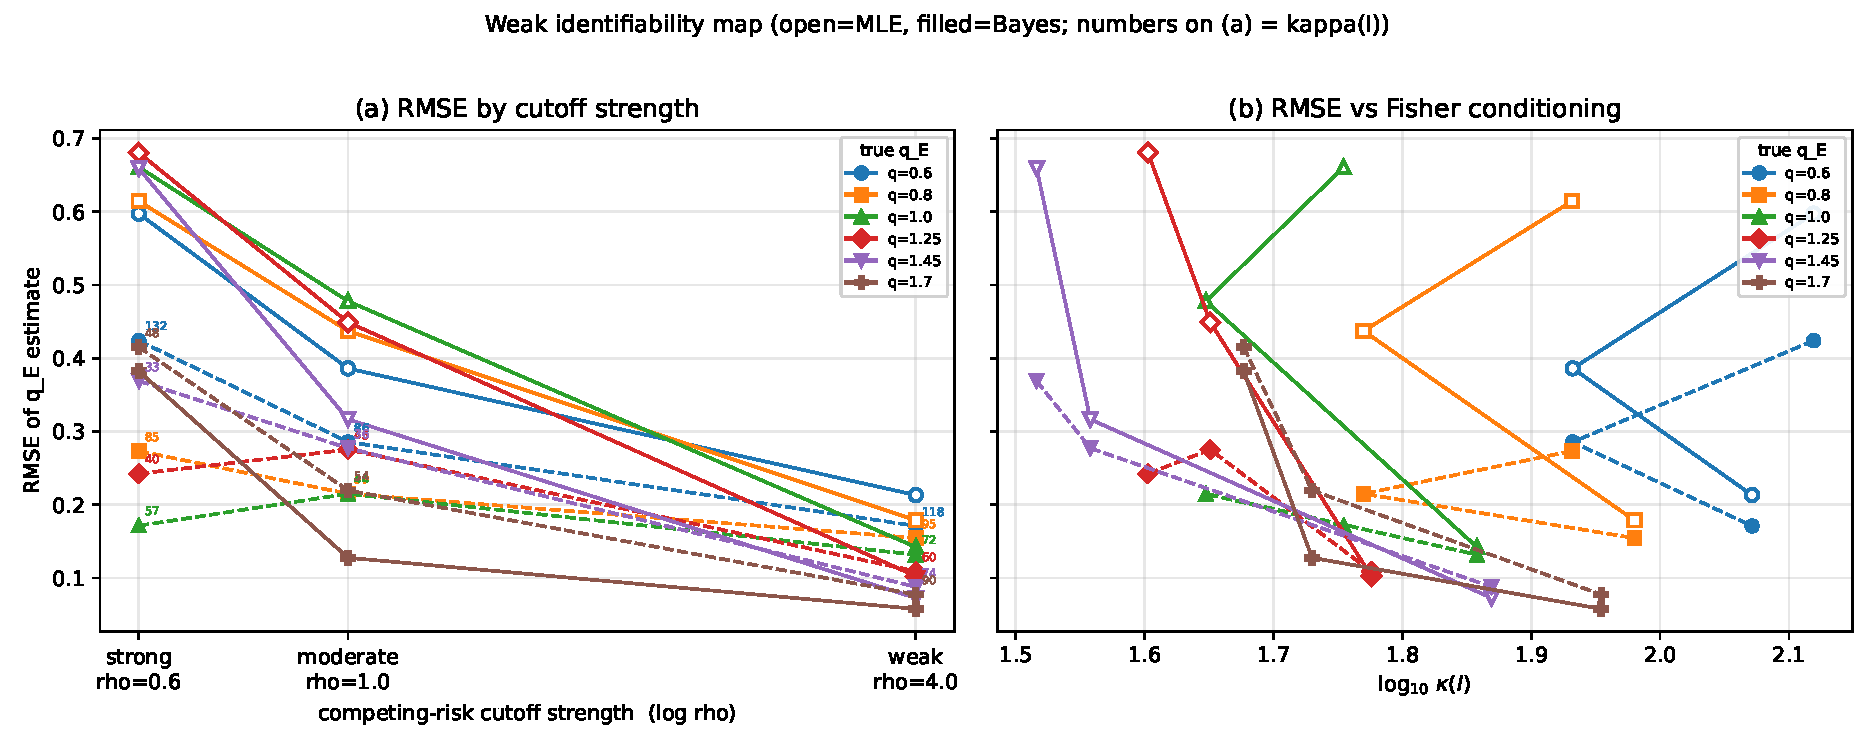
\includegraphics[width=.95\textwidth]{../figures/fig7_weak_id_map.pdf}
\caption{Weak-identifiability map. Across true $q$, the observed
information ($\det\bm I$, smallest eigenvalue $\lambda_{\min}$, condition
number $\kappa$) and the target-cause event fraction
$\mathrm{frac}_{\rm event}$ improve monotonically as truncation weakens,
and the MLE RMSE($q$) tracks the resulting information scarcity. MLE RMSE:
open circles, solid line; Bayes RMSE: filled circles, dashed line.}
\label{fig:weakmap}
\end{figure*}

\subsubsection{Recovery of the scale and shape $\eta,\beta$}\label{sec:etasupp}
Table~\ref{tab:etasupp} reports the recovery of $\eta$ and $\beta$ in
addition to $q$ ($R=30$, Monte Carlo standard error $\approx0.04$). Under
weak truncation all three parameters are recovered cleanly: the $\eta$
bias is single-digit and its RMSE $10$--$13$ (on the $100$-unit median-life
scale), and the $\beta$ bias is small throughout. Under \emph{strong}
truncation, by contrast, $\eta$ becomes severely distorted---for
$q=1.45$ strong the MLE $\eta$ RMSE is $\approx87$---but the Bayesian
interval is correspondingly wide and still covers the truth
($\approx0.9$). The $\beta$ estimates remain stable. One further,
regime-specific pathology appears for the bounded $q=0.6$ under strong
truncation: the support endpoint $T_{\max}$ is occasionally estimated as
infinite, i.e.\ the posterior escapes to $q\ge1$, because the bounded mode
is essentially unidentifiable when almost no units fail from it. This is
consistent with the conservative, wide bounded-regime intervals noted
earlier.

\begin{table}[h]
\centering
\caption{Bayesian recovery of $q,\eta,\beta$ (bias, RMSE, $95\%$
coverage; $n=200$, $R=30$). $\eta$ is severely distorted only under strong
truncation, where the wide interval still covers the truth.}
\label{tab:etasupp}
\small
\begin{tabular}{llccc}
\toprule
Condition & Par. & Bias & RMSE & Coverage\\
\midrule
$q=1.45$ weak  & $q$    & $-0.05$ & $0.09$ & $0.90$\\
               & $\eta$ & $+6.2$  & $13.5$ & $0.93$\\
               & $\beta$& $-0.07$ & $0.20$ & $0.97$\\
$q=1.45$ strong& $q$    & $-0.31$ & $0.39$ & $0.93$\\
               & $\eta$ & $+38.5$ & $50.6$ & $0.90$\\
               & $\beta$& $-0.11$ & $0.31$ & $0.90$\\
$q=0.6$ weak   & $q$    & $-0.01$ & $0.15$ & $0.77$\\
               & $\eta$ & $-1.1$  & $9.7$  & $0.77$\\
               & $\beta$& $-0.00$ & $0.15$ & $0.77$\\
\bottomrule
\end{tabular}
\end{table}

The computational comparison (Figure~\ref{fig:eff}) benchmarks four
samplers on a representative strongly truncated data set ($q=1.45$):
random-walk Metropolis, adaptive Metropolis, a preconditioned HMC with a
fixed trajectory length, and NUTS. When the random walk is given the exact
posterior covariance estimated from the MLE Hessian, a choice that
deliberately favours it, its wall-clock efficiency ($92$ effective samples
per second) matches NUTS ($90$). In this six-dimensional,
well-preconditioned setting NUTS therefore does not gain in effective
samples per second.

Its advantage lies elsewhere. First, NUTS adapts its mass matrix during
warm-up and needs no externally supplied covariance, whereas the
competitive Metropolis result depends on that precomputed input. Second,
the fixed-trajectory HMC over-integrates (acceptance $1.00$) and obtains
only $0.091$ effective samples per gradient evaluation, about half the
$0.179$ attained by NUTS, which selects the trajectory length
automatically. NUTS also remains reliable from dispersed starts and as
the dimension or anisotropy grows, where a single fixed-covariance
proposal deteriorates.

As an external sanity check, we fit the ordinary-Weibull ($q=1$)
competing-risks baseline on the voltage data with a mature
implementation (PyMC 6.3.2, ArviZ 1.3.0; dense-mass NUTS with dual
averaging): it gives zero divergent transitions, $\hat R_{\max}=1.002$,
bulk effective sample size $1382$, and about $81$ effective samples per
second on pure sampling (the $77$ s wall time includes a one-time
just-in-time compilation). Our own NUTS, on the strictly harder
six-parameter q-Weibull posterior, attains about $129$ effective samples
per second with $\hat R_{\max}\approx1.004$, i.e.\ throughput of the same
order as a specialised library on a smaller, easier model.

\begin{figure*}[h]
\centering
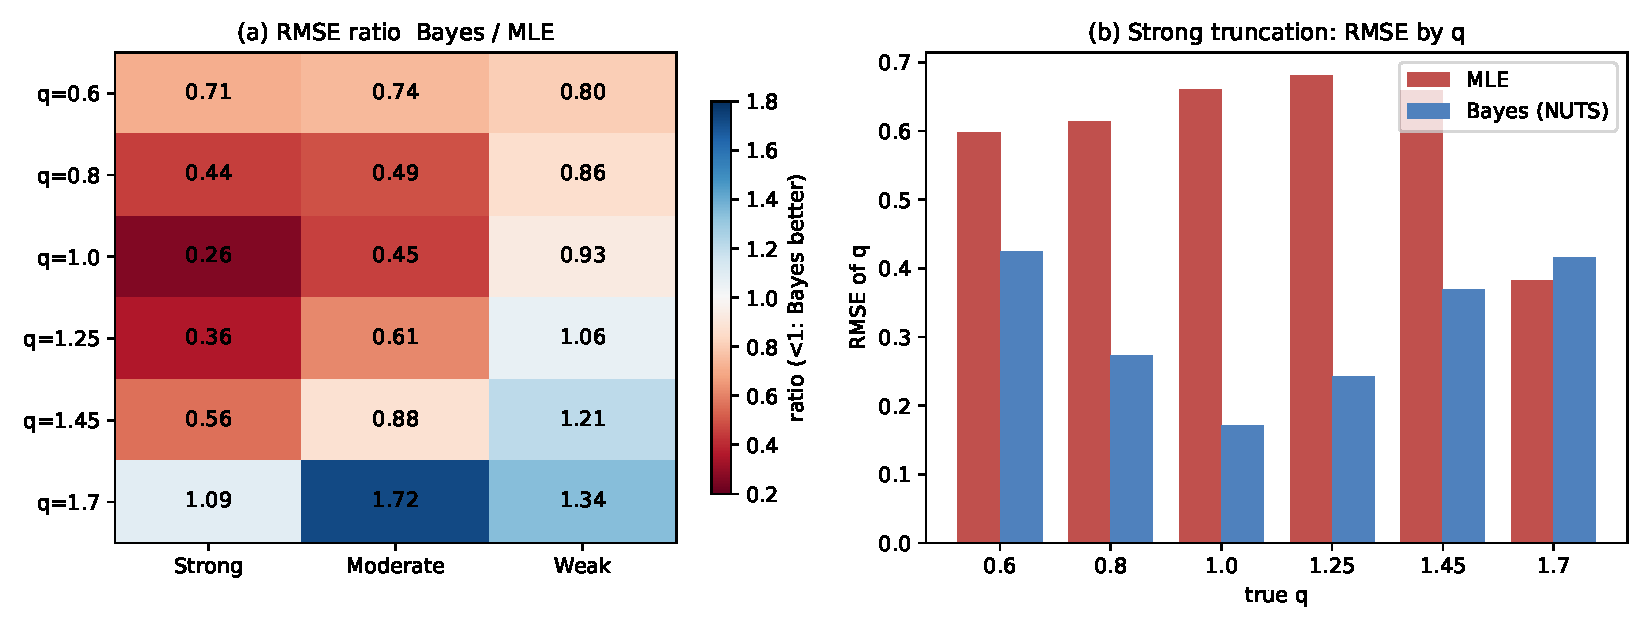
\includegraphics[width=.95\textwidth]{../figures/fig4_sim_performance.pdf}
\caption{(a) RMSE ratio Bayes/MLE across $q$ and truncation (red: Bayes
better, blue: MLE better); (b) RMSE under strong truncation. Bayesian
regularisation helps mainly under strong truncation with moderate
departures from $q=1$.}
\label{fig:perf}
\end{figure*}

\begin{figure*}[h]
\centering
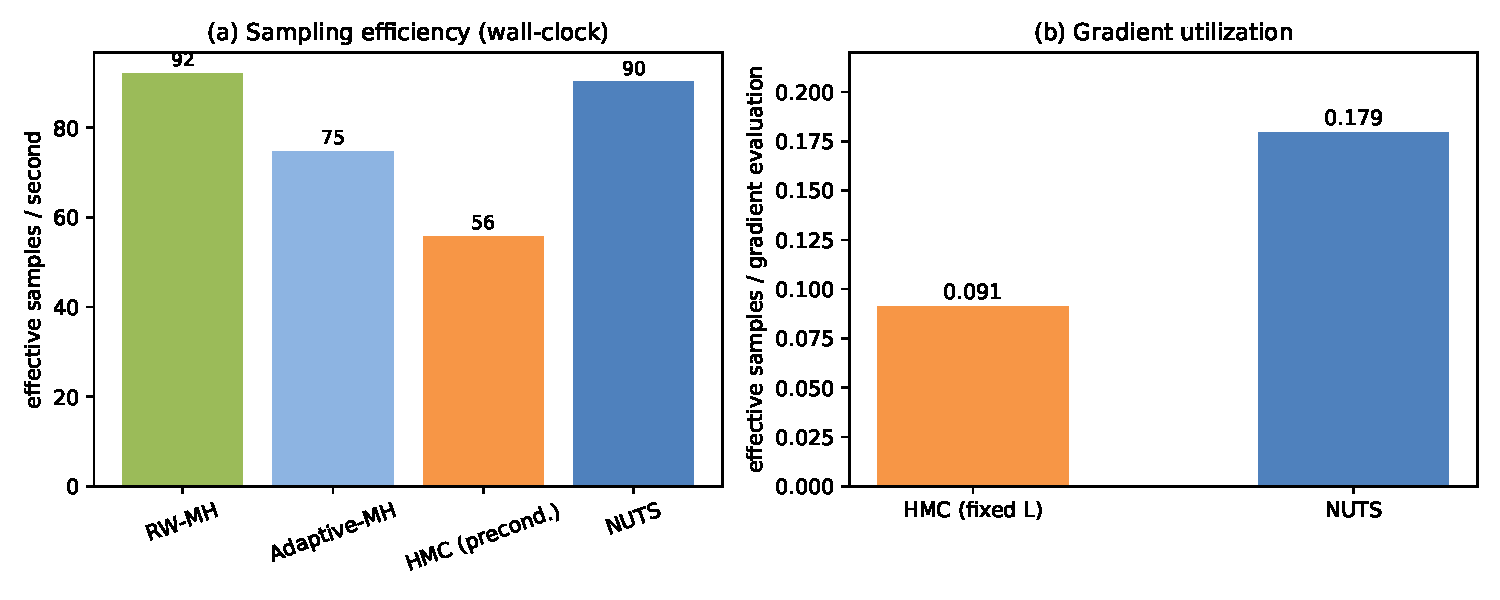
\includegraphics[width=.8\textwidth]{../figures/fig5_efficiency.pdf}
\caption{(a) Effective samples per second for four samplers; a
covariance-preconditioned random walk matches NUTS when given the exact
covariance. (b) Effective samples per gradient evaluation; NUTS uses
gradients about twice as efficiently as a fixed-trajectory HMC.}
\label{fig:eff}
\end{figure*}

\begin{figure}[h]
\centering
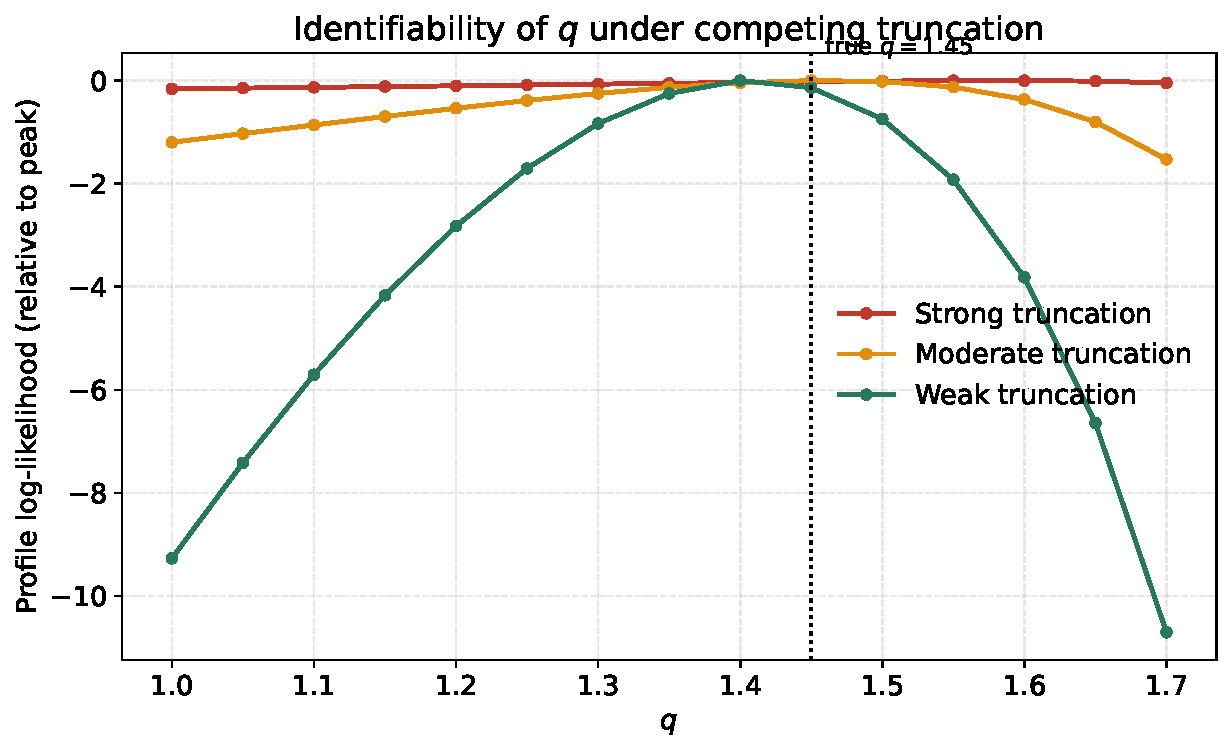
\includegraphics[width=\linewidth]{../figures/fig6_profile_q.pdf}
\caption{Profile log-likelihood of $q$ under strong, moderate, and weak
competing truncation. Early competing failure broadens the profile and
weakens identifiability; with weak truncation the profile sharpens at the
true value.}
\label{fig:profile}
\end{figure}

\subsection{Sensitivity analyses}\label{sec:sens}
We first vary the prior on $q$, reusing the same strongly truncated data
sets ($q=1.45$, $R=40$). The default $\mathcal N(1,0.5^2)$ gives the best
balance (RMSE $0.39$, coverage $0.95$). A tighter
$\mathcal N(1,0.25^2)$ under-covers ($0.72$) with a narrow interval, a
wider $\mathcal N(1,1^2)$ raises the RMSE to $0.49$ but still improves on
the MLE ($0.66$), showing that the gain is not solely the effect of
shrinkage, and a flat $\mathcal U(-1,2)$ gives an unstable point estimate
(RMSE $1.05$) although its wide interval still covers the truth ($0.95$).
With no regularisation the weakly identified posterior is dominated by the
boundary. On the voltage data the early-mode posterior becomes harder to
sample as the prior widens (more divergent transitions), yet under every
prior the $95\%$ interval for $q_E$ contains $1$; the absence of strong
heavy-tail evidence therefore does not rely on a prior centred at the
Weibull value.

The boundary threshold is assessed on the bounded $q=0.6$,
strong-truncation design ($R=40$, Table~\ref{tab:barr}). Posterior
summaries are identical for $\varepsilon_s=10^{-3},10^{-4},10^{-5}$ (bias
$0.38$, RMSE $0.42$, coverage $0.97$, interval width $1.47$), and
$\varepsilon_s=10^{-2}$ differs only marginally. The smallest inner factor
at the fitted parameters is about $0.49$, so the ramp is inactive at every
data point; the threshold changes only the frequency of divergent
transitions in the unobserved near-wall region, not the estimates.

\begin{table}[h]
\centering
\caption{Sensitivity to the smooth-barrier threshold $\varepsilon_s$ on
the bounded $q=0.6$, strong-truncation design ($R=40$).}
\label{tab:barr}
\small
\begin{tabular}{cccccc}
\toprule
$\varepsilon_s$ & Bias & RMSE & Coverage & Interval width & Divergences\\
\midrule
$10^{-2}$ & $0.39$ & $0.44$ & $0.97$ & $1.49$ & $0.12$\\
$10^{-3}$ & $0.38$ & $0.42$ & $0.97$ & $1.47$ & $3.02$\\
$10^{-4}$ & $0.38$ & $0.42$ & $0.97$ & $1.47$ & $3.40$\\
$10^{-5}$ & $0.38$ & $0.42$ & $0.97$ & $1.47$ & $3.40$\\
\bottomrule
\end{tabular}
\end{table}

\paragraph{Prior centre $\mu_q$.}\label{sec:priorcenter}
Because the default prior is centred at the ordinary Weibull value
($\mu_q=1$), we checked how the regularisation target affects the strongly
truncated, heavy-tailed case ($q_{\rm true}=1.45$, $n=200$, $R=30$,
$\sigma_q=0.5$). Centring at $\mu_q=0.8$ gives bias $-0.479$, RMSE
$0.534$, coverage $0.90$; the default $\mu_q=1.0$ gives $-0.311$, $0.388$,
$0.93$; and $\mu_q=1.2$ gives $-0.207$, $0.302$, $0.97$. The bias and RMSE
improve monotonically as the centre approaches the truth, and the
coverage rises to near-nominal. This confirms that the remaining downward
shrinkage bias under strong truncation (about $-0.31$ at the default
centre) is a property of anchoring at $q=1$, not a sampling artefact; in
practice the centre should be placed near the physically expected tail
behaviour whenever prior information exists.

\paragraph{Upper-truncation boundary fraction.}\label{sec:boundf}
For the bounded regime the location of the observational window relative
to the support endpoint matters. Define $f=\max_i t_i/T_{\max}$, the
fraction of the theoretical endpoint reached by the largest observed time
($q=0.6$, weak truncation, $n=200$, $R=20$). At $f=0.5$ (about $35\%$
censoring) the MLE biases $q$ upward by $+0.13$ and the Bayes estimate by
$+0.28$, with coverage falling to $0.65$; at $f=0.7$ the bias is $+0.05$
and coverage $0.85$; for $f\ge0.85$ the estimates return to the
weak-truncation baseline (bias $\approx0$, coverage $\approx0.75$). Heavy
upper truncation against a bounded support thus pushes the bounded $q$
upward and degrades coverage, because the finite endpoint is essentially
unobserved.

\paragraph{Sample size.}\label{sec:n}
Finally, Figure~\ref{fig:n_effect} varies $n$ under the hardest design
($q_{\rm true}=1.45$, strong truncation). The MLE RMSE stays on a weak-identification
plateau---$0.73$, $0.78$, $0.76$ for $n=50,100,200$---and collapses only at
$n=500$ to $0.20$; the Bayesian RMSE is flatter and better-calibrated
($0.37$, $0.39$, $0.40$, $0.26$) with coverage at least $0.92$ throughout.
This shows that, under strong competing truncation, increasing the sample
size in the hundreds does not by itself restore identifiability: the
regularisation and the honest interval are what stabilise inference until
the information (sample size and/or observed tail) becomes large. The
$n=500$ point uses only $R=12$ replicates (Monte Carlo standard error
$\approx0.063$). Figure~\ref{fig:n_effect} uses distinct black line styles
and markers (solid circle, dashed square, dotted triangle, dash-dot
diamond) so it prints unambiguously in greyscale.

\begin{figure}[h]
\centering
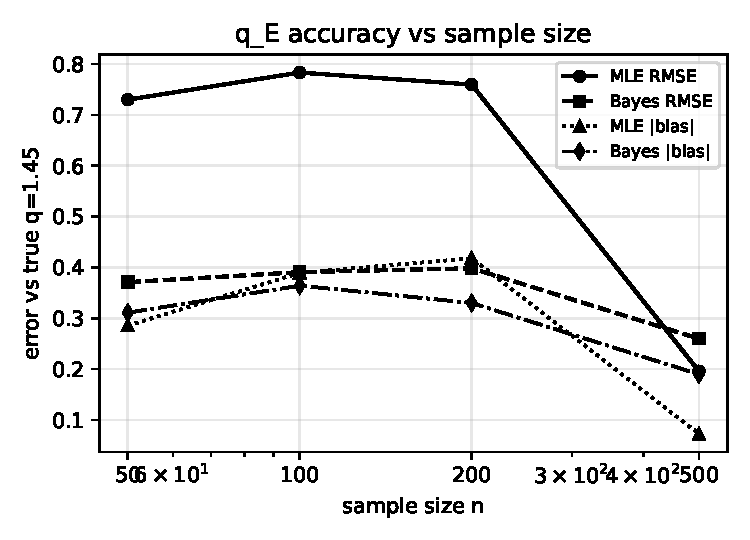
\includegraphics[width=\linewidth]{../figures/fig9_n_effect.pdf}
\caption{Estimation error versus sample size under strong truncation
($q=1.45$). The MLE RMSE stays on a weak-identification plateau for
$n=50$--$200$ and drops only at $n=500$; the Bayesian RMSE is flatter and
its coverage stays at least $0.92$. Distinct black line styles and markers
are used for greyscale legibility.}
\label{fig:n_effect}
\end{figure}

% =====================================================================
\section{Application to high-voltage stress-test data}\label{sec:app}
% =====================================================================

\subsection{Data description}\label{sec:data}
We analyse the \texttt{voltage} data from a high-voltage stress test of
generator armature bars \cite{doganaksoy2002}, distributed with the
\texttt{weibulltools} package \cite{weibulltools}. Fifty-eight independent units were
followed until failure or censoring; $18$ failed from an \emph{early} mode
(E), $27$ from a \emph{degradation} mode (D), and $13$ were right-censored.
Figure~\ref{fig:data} shows the event times: E failures are concentrated at
short times while D failures occur later, consistent with two distinct
mechanisms.

\begin{figure}[h]
\centering
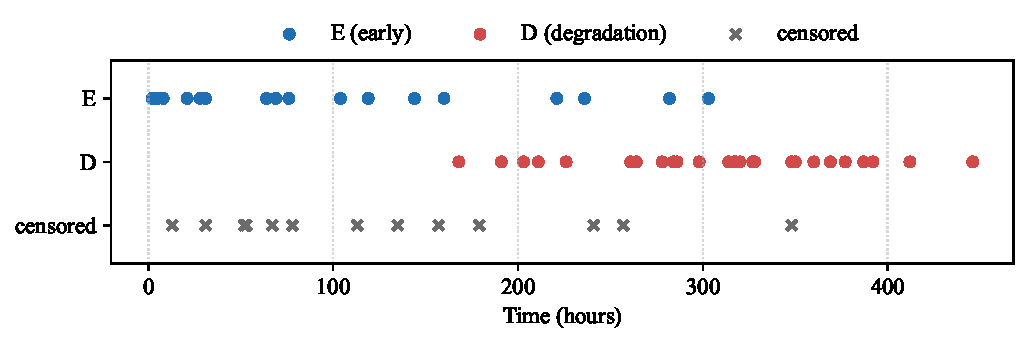
\includegraphics[width=\linewidth]{../figures/fig1_data.pdf}
\caption{Event and censoring times by failure mode for the voltage data.}
\label{fig:data}
\end{figure}

\subsection{Model comparison and posterior inference}\label{sec:mcomp}
Table \ref{tab:models} compares a single Weibull, a Weibull competing-risks
model, and a q-Weibull competing-risks model by maximum likelihood.
\begin{table}[h]
\centering
\caption{Maximum-likelihood comparison for the voltage data.}
\label{tab:models}
\small
\begin{tabular}{lcccc}
\toprule
Model & No.\ params & Log-lik. & AIC & BIC\\
\midrule
Single Weibull & 2 & $-292.53$ & 589.06 & 593.18\\
Weibull CR & 4 & $-287.07$ & \textbf{582.13} & \textbf{590.37}\\
q-Weibull CR & 6 & $-287.05$ & 586.10 & 598.46\\
\bottomrule
\end{tabular}
\end{table}

Allowing two causes is strongly supported: the likelihood-ratio statistic
against the single Weibull is $10.92$ ($p\approx0.004$). Adding $q$, however,
is not significant ($2\Delta\ell=0.038$, $p\approx0.98$), and the q-Weibull
model is penalised by AIC \cite{akaike1974} and BIC \cite{schwarz1978}.
The Bayesian posterior (Table
\ref{tab:post}, Figure~\ref{fig:qpost}) tells a consistent and nuanced
story. The early mode shows a weak heavy-tail signal: the posterior is
shifted above one with $\Pr(q_E>1)\approx0.76$, but its interval includes
one, whereas the degradation mode is centred at $q_D\approx0.97$ and is
adequately represented by an ordinary Weibull. We report this uncertainty
transparently rather than claim heavy tails the data do not establish.
For the early mode the characteristic life $\eta_E$ is also only weakly
determined (95\% interval $91$--$2429$ h), because the scale is confounded
with the heavy-tail shape over the short early-mode window; the
degradation-mode scale $\eta_D$ is estimated much more precisely
($297$--$409$ h).

\begin{table}[h]
\centering
\caption{Bayesian posterior summaries for the q-Weibull competing-risks
model (NUTS, target acceptance $0.90$).}
\label{tab:post}
\small
\begin{tabular}{lccc}
\toprule
Parameter & Median & 95\% interval & $\Pr(q>1)$\\
\midrule
$q_E$ & 1.23 & $[0.64,\,1.71]$ & 0.76\\
$\eta_E$ (h) & 599 & $[91,\,2429]$ & --\\
$\beta_E$ & 0.67 & $[0.44,\,0.98]$ & --\\
$q_D$ & 0.97 & $[0.51,\,1.38]$ & 0.46\\
$\eta_D$ (h) & 350 & $[297,\,409]$ & --\\
$\beta_D$ & 5.23 & $[3.61,\,7.60]$ & --\\
\bottomrule
\end{tabular}
\end{table}

\subsection{Bayesian Weibull baseline.}\label{sec:weibbaseline}
Restricting both causes to ordinary Weibulls in the Bayesian fit ($q=1$,
four parameters) gives a regularised comparison: $\eta_E=925$ h ($95\%$
interval $474$--$2788$), $\beta_E=0.68$ ($0.43$--$0.98$),
$\eta_D=345$ h ($320$--$376$), and $\beta_D=5.31$ ($3.80$--$6.92$), with
no divergent transitions and posterior log-likelihood median $-289.1$. The
q-Weibull Bayesian fit reaches no higher posterior log-likelihood,
consistent with the likelihood-ratio result ($2\Delta\ell=0.038$). Freeing
$q$ therefore adds no predictive value on these data, and the Weibull fit
is both more parsimonious and numerically cleaner. The framework can
represent a heavy tail when that tail is observed, as the simulation
shows, but here it correctly withholds that interpretation.

\begin{figure}[h]
\centering
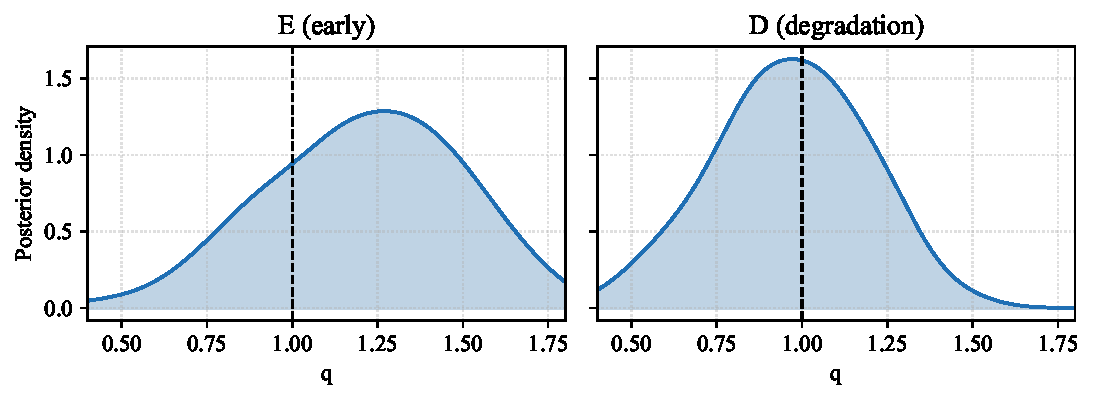
\includegraphics[width=\linewidth]{../figures/fig2_qpost.pdf}
\caption{Posterior density of $q$ for the early and degradation modes; the
dashed line marks $q=1$ (ordinary Weibull).}
\label{fig:qpost}
\end{figure}

\subsection{Cumulative incidence and cause probabilities}\label{sec:cif}
Figure~\ref{fig:ciffig} shows the posterior system reliability and CIFs. The
estimated eventual cause probabilities are $0.37$ for E (95\% interval
$0.26$--$0.48$) and $0.63$ for D ($0.52$--$0.74$), close to the observed
failure proportions ($18/45=40\%$, $27/45=60\%$). At the largest observed
time ($446$ h), the system reliability is $0.018$, with $\CIF_E=0.37$ and
$\CIF_D=0.62$. For every posterior draw the CIFs and system reliability
satisfy $\CIF_E(t)+\CIF_D(t)+R_{\rm sys}(t)=1$ up to a numerical integration
error below $0.01$; we report posterior means, which remain additive, rather
than separately computed medians. The fitted system reliability closely
tracks the non-parametric Kaplan--Meier estimate \cite{kaplanmeier1958},
supporting the parametric model.

\begin{figure}[h]
\centering
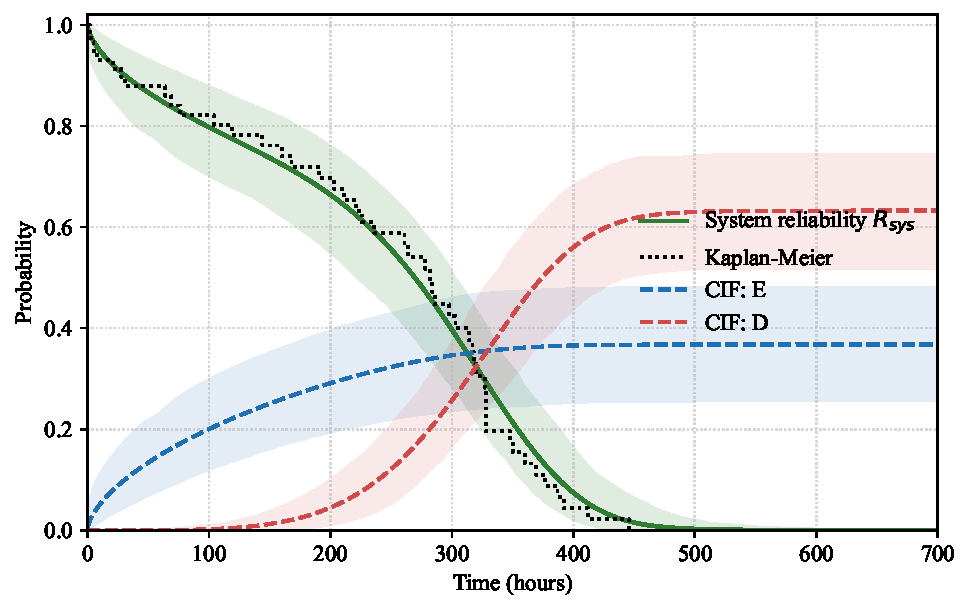
\includegraphics[width=\linewidth]{../figures/fig3_cif.pdf}
\caption{Posterior system reliability and cause-specific cumulative
incidence functions with uncertainty bands, with Kaplan--Meier comparison.}
\label{fig:ciffig}
\end{figure}

\subsection{Posterior predictive check}\label{sec:ppc}
To verify that the fitted model can reproduce the salient features of the
data, we drew $B=300$ posterior replicates (re-applying the observed
censoring times) and compared observed statistics to their posterior
predictive distribution (Figure~\ref{fig:ppc}). The observed $18$
early-mode failures sit inside the $95\%$ predictive interval $[10,\,28.5]$
(median $19$), the $27$ degradation-mode failures inside $[21,\,38]$
(median $29$), and the largest observed lifetime $446$ h inside
$[390,\,549]$ h (median $442$ h). The cumulative incidences at the last
observed time agree: $\CIF_E(446)=0.346$ versus predictive $[0.197,0.549]$,
and $\CIF_D(446)=0.617$ versus $[0.431,0.799]$. The modelled system
reliability over $50$--$400$ h lies entirely within the $95\%$ predictive
band. No observed statistic falls outside its predictive interval, so the
q-Weibull competing-risks model reproduces the failure counts, the range
of lifetimes, and the cause-specific accumulation; the PPC therefore does
not reveal a structural misspecification, while it remains consistent with
the earlier conclusion that the heavy-tail signal for the early mode is
weak.

\begin{figure}[h]
\centering
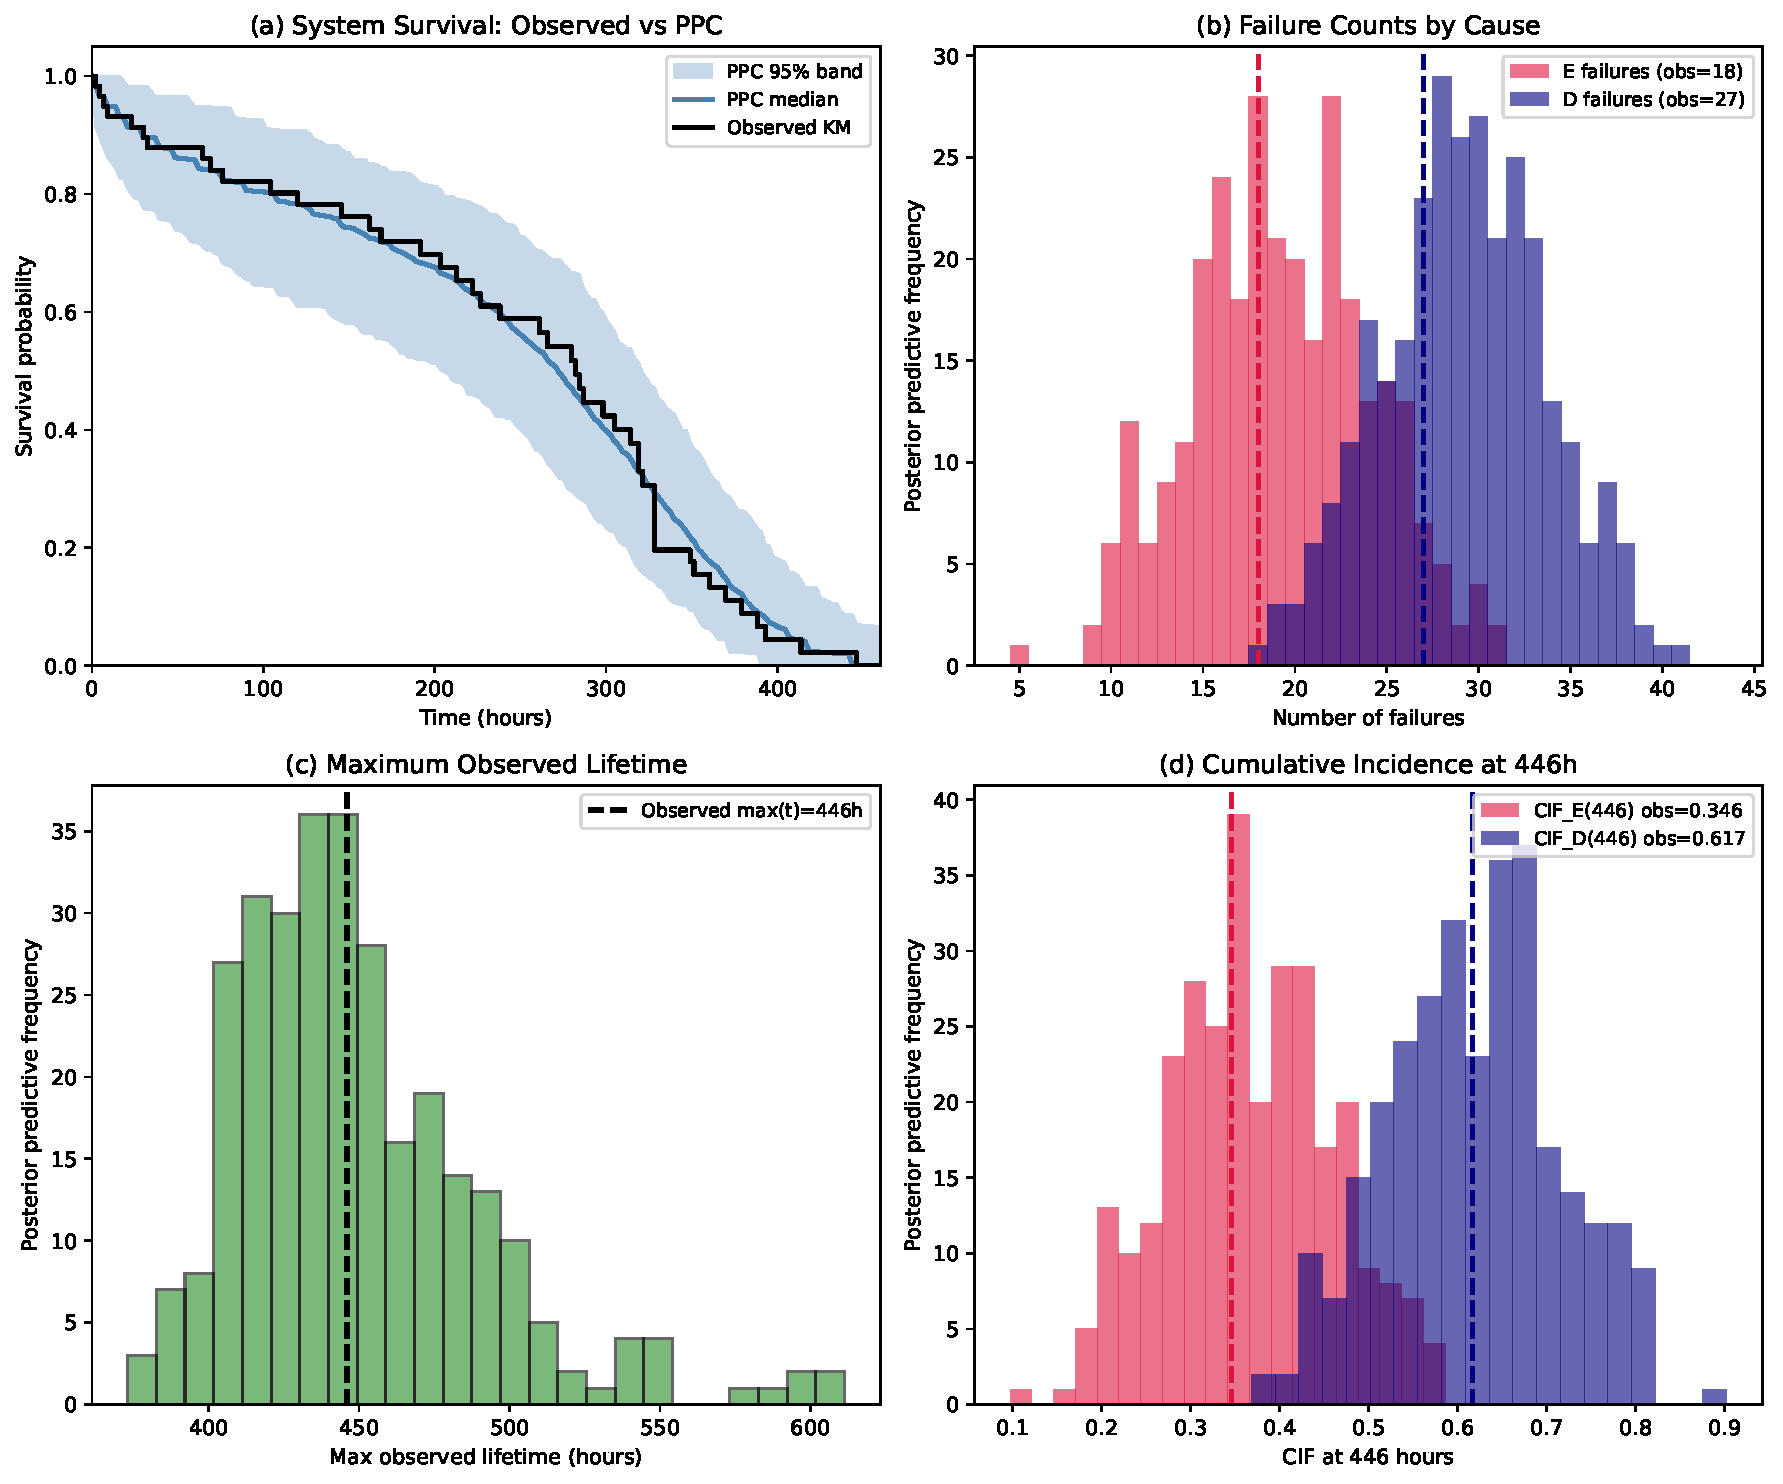
\includegraphics[width=\linewidth]{../figures/fig10_ppc.pdf}
\caption{Posterior predictive check for the voltage data ($B=300$ draws).
Observed summaries (vertical dashed lines) lie inside their $95\%$
predictive intervals (shaded bands / histograms) for the failure counts,
the maximum lifetime, the cause-specific CIFs at $446$ h, and the system
reliability over $50$--$400$ h.}
\label{fig:ppc}
\end{figure}

% =====================================================================
\section{Discussion}\label{sec:disc}
% =====================================================================
The findings clarify both the value and the limits of Bayesian inference for
q-Weibull competing risks. The central mechanism is identifiability: the
entropic parameter $q$ is read mainly from the tail, and a competing cause
that truncates the tail removes exactly the information needed to estimate
it. The resulting likelihood is broad and asymmetric, and its shape differs
by regime. Heavy-tailed $q>1$ is identifiable once the tail is observed,
whereas bounded $q<1$ is intrinsically harder because $q$, $\beta$, and the
support endpoint are partially confounded over any finite observation window.

Bayesian regularisation is beneficial precisely in the limited-information
regime: a weakly informative prior centred at the ordinary Weibull reduces
estimator variance (and RMSE) without claiming to remove the systematic
truncation bias, and the full posterior communicates uncertainty that a
Wald interval cannot. When the data are informative, the same broad prior
recedes and the likelihood dominates, so the method does not impose
shrinkage where it is unwarranted. We caution against interpreting a
posterior shifted above one as proof of heavy tails without an interval that
excludes one, as the voltage application illustrates.

On the computational side, NUTS with an analytic gradient, Hessian
preconditioning, and the smooth barrier gives reliable, high-ESS inference
even at the bounded support wall where naive samplers freeze.

A key limitation is the assumption of independent latent cause-specific
times. To gauge its effect we simulated data from a shared-gamma-frailty
model (so the two causes are dependent) but fitted the \emph{wrong}
independent q-Weibull competing-risks Bayes model ($q_{\rm true}=1.45$,
strong truncation, $n=200$, $R=20$). With independent data the bias in
$q_E$ is $-0.30$ (RMSE $0.39$, coverage $0.90$); under mild dependence
(frailty variance $\nu=5$) it shrinks to $-0.08$ (RMSE $0.23$, coverage
$1.00$); and under stronger dependence ($\nu=2$) it flips to $+0.25$
(RMSE $0.31$, coverage $0.80$). Ignoring positive frailty dependence thus
moves the $q_E$ bias from negative to positive and degrades coverage to
$0.80$: the independent-cause assumption is acceptable under weak
dependence but should be relaxed, e.g.\ with shared-frailty or
copula-cause models, when dependence is suspected. Other limitations
include the choice of prior scale and the modest sample size of the
application.
Natural extensions are accelerated life tests with stress-dependent scale
parameters, hierarchical and covariate-dependent models, dependent causes,
and robust inference under contamination \cite{qre70113}; a recent survey of
q-Weibull reliability applications is given by \cite{ieeetr2025qw}. We also
refer to \cite{gelman2014} for the general Bayesian workflow.

% =====================================================================
\section{Conclusion}\label{sec:concl}
% =====================================================================
We developed a unified Bayesian framework for q-Weibull competing risks,
computed by NUTS in weakly coupled, unconstrained coordinates
$(q,\log\eta,\log\beta)$ with an analytic gradient and a smooth barrier for
the bounded support wall. Across the bounded, Weibull, and heavy-tailed regimes, the simulation
showed that competing truncation weakens the identifiability of the tail
parameter $q$, and it mapped where Bayesian shrinkage helps: it stabilises
estimation and yields honest uncertainty intervals when information is
scarce and $q$ departs only moderately from one, whereas the likelihood
dominates when the tail is observed or $q$ lies far from the centre. On
the computational side, NUTS adapts its mass matrix automatically and
uses gradient evaluations about twice as efficiently as a
fixed-trajectory HMC; it matches a covariance-preconditioned random walk
only in the special case where that walk is handed the exact posterior
covariance.
Applied to high-voltage stress-test
data, the method established significant competing risks, identified a weak
and uncertain heavy-tail signal in the early mode, and confirmed an
ordinary Weibull for the degradation mode, reporting the non-significance
of $q$ without overstatement. The framework provides a practical and honest
basis for q-Weibull competing-risks analysis and a foundation for
accelerated-test and hierarchical extensions.

\bmsubsection*{Author Contributions}
Huirong Cao: conceptualisation, methodology, software, formal analysis,
visualisation, writing--original draft. Fuchang Wang: supervision,
methodology, writing--review and editing.

\bmsubsection*{Acknowledgments}
The authors thank the editor and the reviewers for comments that
substantially improved the paper.

\bmsubsection*{Financial Disclosure}
This research received no external funding.

\bmsubsection*{Conflicts of Interest}
The authors declare no conflicts of interest.

\bmsubsection*{Data Availability}
The \texttt{voltage} data are publicly available through the
\texttt{weibulltools} R package \cite{weibulltools}. All simulation,
fitting, plotting, and result-generation code, together with the
machine-readable result files used in this paper, is released as a
reproducible research package on GitHub
(\texttt{https://github.com/fzmath/qweibull-cr}). The package has the
structure
\begin{verbatim}
qweibull-cr/
  code/      Python (numpy/scipy/pandas/matplotlib/pymc) scripts:
             nuts.py, bayes_model.py, cr_bayes_model.py,
             penalized_mle.py, fisher_info.py, param_compare.py,
             pymc_baseline.py, sim_eta_beta.py,
             prior_center_sensitivity.py, boundary_fraction.py,
             sample_size.py, ppc_voltage.py, dependent_cr.py
  data/      simulation result JSONs, voltage.csv, posterior chains
  figures/   fig1..fig10 (PDF and PNG)
  paper/     main.tex, references.bib, USG.cls, build script
\end{verbatim}
Results are regenerated by running the \texttt{code/} scripts in order and
compiling \texttt{paper/main.tex} with XeLaTeX (Section~\ref{app:build}).

\appendix
\section{Details of the No-U-Turn sampler}\label{app:nuts}
This appendix supplies the implementation details summarised in
Algorithm~\ref{alg:nuts}. We use the standard NUTS construction of
\cite{hoffman2014nuts,carpenter2017stan}. Given a current point
$\bm x$ and a momentum draw $\bm r\sim\mathcal N(\bm0,\bm M)$, a slice
variable $u\sim\mathrm{Uniform}(0,\exp[-H(\bm x,\bm r)])$ defines the set
of admissible points. The tree is built by recursion: at each doubling the
leapfrog trajectory is extended by one more step in the current direction
from either the leftmost or the rightmost leaf, and the proposal is chosen
uniformly among the leaves whose joint density exceeds $u$. The recursion
stops when (i) the two outermost leaves double back on themselves
(U-turn, $(\bm x^{+}-\bm x^{-})^{\top}\bm r<0$), (ii) a leapfrog step
produces a divergent transition (the squared Hamiltonian jump exceeds the
divergence threshold, calibrated from the energy distribution), or (iii) a
maximum tree depth (we use $10$) is reached. Divergent transitions are
rejected for the target estimate but retained for diagnostics.

During warmup, the step size $\varepsilon$ is tuned by primal-dual
averaging \cite{hoffman2014nuts} toward a target acceptance probability
$\delta=0.85$--$0.90$: a dual variable adapts $\log\varepsilon$ with a
decreasing gain, and the running average is what is finally used, which
stabilises the adaptation. The mass matrix $\bm M$ is set once from the
Hessian preconditioner below; re-estimation from the first half of warmup
draws is implemented but found unnecessary here.

\section{Analytic gradient and Hessian preconditioner}\label{app:hess}
The log-posterior gradient used in the leapfrog steps is the analytic
expression of Section~\ref{sec:post}. For each cause, the raw likelihood
gradients $(g_q,g_\lambda,g_\beta)$ of Equations \eqref{eq:f}--\eqref{eq:h}
are obtained by differentiating \eqref{eq:Lj} term by term, using the
inner factor $u(t)=1-(1-q)\lambda t^\beta$ and its derivatives; the
$q=1$ limit \eqref{eq:q1lim} removes the apparent $0/0$ singularity. The
cause-separable form \eqref{eq:Lj} means the six-parameter gradient is the
concatenation of two three-cause gradients. These analytic derivatives agree
with central finite differences to relative error below $10^{-8}$.

The preconditioning mass matrix is built from the negative Hessian
$\bm H=-\nabla^{2}\log p(\bm x)$ evaluated at the posterior mode (or,
before fitting, at the MLE). Because the raw Hessian can be indefinite or
ill-conditioned in the weakly identified directions, we regularise it in
one of two equivalent ways: (i) add a small ridge, $\bm M=\bm H+\varepsilon
\bm I$ with $\varepsilon=10^{-3}\,\mathrm{tr}(\bm H)/d$, and (ii) an
eigenvalue clip, $\lambda_i\leftarrow\max(\lambda_i,\,\lambda_{\max}/\kappa_{\max})$
with $\kappa_{\max}=10^{4}$, which prevents any direction from being too
flat (which would inflate the leapfrog step) or too steep (which would
shrink it). The draw $\bm r\sim\mathcal N(\bm0,\bm M)$ and the position
update $\bm x\leftarrow\bm x+\varepsilon\bm M^{-1}\bm r$ then use the
symmetrised, regularised factorisation. This is a local preconditioner to
reduce posterior anisotropy, not an exact posterior covariance
(Section~\ref{sec:adapt}).

\section{Reproducing the build}\label{app:build}
The manuscript is compiled with XeLaTeX against the Wiley NJD
\texttt{USG} class:
\begin{verbatim}
xelatex -interaction=nonstopmode main.tex
bibtex main
xelatex -interaction=nonstopmode main.tex
xelatex -interaction=nonstopmode main.tex
\end{verbatim}
Python 3.10+ with \texttt{numpy}, \texttt{scipy}, \texttt{pandas},
\texttt{matplotlib}, and (for the external baseline only) \texttt{pymc}
6.x / \texttt{arviz} 1.x reproduces all numbers and figures; the result
JSONs in \texttt{data/} are the exact sources of every table entry above.

\bibliography{references}

\begin{biography}{}{%
\author{Fuchang Wang} is a Professor at the University of Emergency
Management, Sanhe, China. His research interests include statistical
computing, machine learning, and artificial intelligence.}
\end{biography}

\begin{biography}{}{%
\author{Huirong Cao} is an Associate Professor in the School of Science at
Langfang Normal University, Langfang, China. Her research interests include
reliability statistics, Bayesian computation, computational actuarial
science, and risk management.}
\end{biography}

\end{document}
